\documentclass[a4paper,10pt]{article}

\usepackage{amsfonts}
\usepackage{amssymb}
\usepackage{latexsym}
\usepackage{graphicx}
\usepackage{amssymb,amsmath}
\usepackage{listings}
\usepackage[titletoc]{appendix}
\usepackage{courier}
\usepackage[countmax]{subfloat}
\usepackage{here}

\linespread{1}

\hoffset -1in \topmargin 0mm \voffset 0mm \headheight 0mm
\headsep0mm
\oddsidemargin  20mm     %   Left margin on odd-numbered pages.
\evensidemargin 20mm     %   Left margin on even-numbered pages.
\textwidth   170mm       %   Width of text line.
\textheight  252mm

\makeatletter
\renewcommand\@openbib@code{%
     \advance\leftmargin  \z@ %\bibindent
      \itemindent \z@
     % Move bibitems close together
     \parsep -0.8ex
     }
\makeatother

\makeatletter
\renewcommand\section{\@startsection {section}{1}{\z@}%
                                   {-3.5ex \@plus -1ex \@minus -.2ex}%
                                   {2.3ex \@plus.2ex}%
                                   {\large\bfseries}}
\makeatother

\makeatletter
\renewcommand\subsection{\@startsection {subsection}{1}{\z@}%
                                   {-3.5ex \@plus -1ex \@minus -.2ex}%
                                   {2.3ex \@plus.2ex}%
                                   {\normalsize\bfseries}}
\makeatother

\begin{document}
\pagestyle{empty}

\begin{center}
{\bf \Large REVISITED BOX COUNTING TECHNIQUE IN BAYESIAN SENSE}
\end{center}

\smallskip
\begin{center}
{\large V\'{a}clav Hubata--Vacek$^1$, David Blatsk\'{y}$^1$, Jarom\'{i}r Kukal$^1$}
\end{center}

\smallskip
\begin{center}
$^1$CTU in Prague, Faculty of Nuclear Sciences and Physical Engineering\\
Department of Software Engineering \\
B\v{r}ehov\'{a} 7, 115 19 Prague 1 \\
Czech Republic\\
hubatvac@fjfi.cvut.cz\\
 ~\\

\end{center}

\bigskip
\noindent Abstract: \textit{}

\vspace*{10pt} \noindent Keywords: \textit{unbiased estimation, Hartley entropy, Shannon entropy, Box Counting}


\bigskip
\section {Introduction }
Fractals are objects, which exceed its topological dimensions and its Hausdorff dimension is not integer. Box Counting method is used for estimating fractal dimension in the form
\begin{equation} 
\label{eq:boxcount}
\ln{C(a)} = A - D_{0}\ln{a},
\end{equation}
where $a>0$ is box size and $C(a)$ is number of covering elements. Capacity dimension $D_{0}$ is estimated as slope of the line which is generated by least square method. These estimate is biased especialy for small values of $a$. Box Counting method can be improved by Bayesian estimation of Hartley entropy $H_{0}$, which offers better estimate of capacity dimension $D_{0}$.

\section {Multinomial Distribution and Naive Entropy Estimates}

Multinomial distrubution model plays main role in investigation of point set structures. Let $n \in \mathbb{N}$ be number of distinguish events. Let $p_{j} > 0$ be probability of $j^{\text{th}}$ event for $j = 1,...,n$ satisfying $ \sum_{j=1}^{n} p_{j} =1$. Then random variable $j$ has multinomial distribution $\text{Mul}(p_{1},...,p_{n})$. After realization of multinomial distribution sample of size $N \in \mathbb{N}$, we can count the events and obtain $N_{j} \in \mathbb{N}_{0}$ as number of $j^{\text{th}}$ event occurences for $j=1,...,n$ satisfying $\sum_{j=1}^{n} N_{j} = N$. Therefore, we define number of various events in sample as $K = \sum_{N_{j}>0} 1 \le \text{min}(n,N)$. Remembering Hartley and Shannon entropy definition as
\begin{equation} 
\label{eq:hnula}
H_{0}=\ln{n},
\end{equation} 
\begin{equation} 
\label{eq:hjedna}
H_{1}=-\sum_{j=1}^{n} p_{j}\ln{p_{j}},
\end{equation}   
we can perform direct but naive estimation of them as
\begin{equation} 
\label{eq:hnulaap}
H_{0,\mbox{\scriptsize{NAIVE}}}=\ln{K},
\end{equation} 
\begin{equation} 
\label{eq:hjednaap}
H_{1,\mbox{\scriptsize{NAIVE}}}=-\sum_{N_{j}>0} \frac{N_{j}}{N}\ln{\frac{N_{j}}{N}}.
\end{equation}   
The main disadvantage of naive estimates is their biasness. Random variable $K= \{ 1,...,n \} $ is upper constrained by $n$, then $\text{E}H_{0,\mbox{\scriptsize{NAIVE}}} = \text{E}\ln{K} < \text{E}\ln{n} = \ln{n} = H_{0}$. Therefore, naive estimate of Hartley entropy $H_{0,\mbox{\scriptsize{NAIVE}}}$ is negative biased. On the other hand, traditional Box Counting Technique is based on this estimate because we plot logarithm of covering element number $C(a) \in \mathbb{N}$ against logarithm of covering element size $a > 0$ and then estimate their dependency in linear form $\ln{C(a)} = A_{0} - D_{0,\mbox{\scriptsize{NAIVE}}}\ln{a}$. Recognizing equivalence $C(a) = K$, we obtain $\ln{C(a)} = \ln{K} = H_{0,\mbox{\scriptsize{NAIVE}}}$ and then $H_{0,\mbox{\scriptsize{NAIVE}}} = A_{0} - D_{0,\mbox{\scriptsize{NAIVE}}}\ln{a}$. Defining $D_{0,\mbox{\scriptsize{NAIVE}}}$ as estimate of capacity dimension and recognizing the occurence of $H_{0,\mbox{\scriptsize{NAIVE}}}$ in Box Counting procedure, we are not suprised to be victims of the bias of Hartley entropy estimate.\\ 
\\*
Similar situation is the case of Shannon entropy estimation. There are several approaches how to decrease the bias of $H_{1,\mbox{\scriptsize{NAIVE}}}$ to be closer to Shannon entropy $H_{1}$. Miller [\ref{bib5}] modified naive estimate $H_{1,\mbox{\scriptsize{NAIVE}}}$ using first order Taylor expansion, which produces
\begin{equation}
\label{eq:miller}
H_{1,\mbox{\scriptsize{M}}}=H_{1,\mbox{\scriptsize{NAIVE}}} + \frac{K-1}{2N}.
\end{equation}
Lately, Harris [\ref{bib5}] improved the formula to
\begin{equation}
\label{eq:harris1h}
H_{1,\mbox{\scriptsize{H}}}=H_{1,\mbox{\scriptsize{NAIVE}}} + \frac{K-1}{2N} + \frac{1}{12N^2} \left( 1 - \sum_{p_{j}>0}\frac{1}{p_{j}} \right)
\end{equation}
Finally, we can estimate information dimension according to relation
\begin{equation} 
\label{eq:hjednaest}
H_{1,\mbox{\scriptsize{EST}}}=A_{1} - D_{1,\mbox{\scriptsize{EST}}} \ln{a}
\end{equation} 
where $H_{1,\mbox{\scriptsize{EST}}}$ is any estimate of $H_{1}$. Therefore, we can also estimate Hausdorff dimension $D_{\mbox{\scriptsize{H}}}$ using inequalities $D_{1} \le D_{\mbox{\scriptsize{H}}} \le D_{0}$ and then also supposing $D_{1,\mbox{\scriptsize{EST}}} \le D_{\mbox{\scriptsize{H}}} \le D_{0,\mbox{\scriptsize{EST}}}$ for any "good" estimates $D_{0,\mbox{\scriptsize{EST}}}$, $D_{1,\mbox{\scriptsize{EST}}}$ of capacity and information dimensions. Next section is oriented to Bayesian estimation of $H_{0}$, $H_{1}$ for $D_{0,\mbox{\scriptsize{EST}}}$ and $D_{1,\mbox{\scriptsize{EST}}}$ evaluations.
\section {Bayesian Estimation of Hartley Entropy}
We suppose uniform distribution of random vector $\vec{p} = (p_{1},...,p_{n})$ satisfying  $p_{j} \ge 0$, $\sum_{j=1}^{n} p_{j} = 1$. Using properties of multinomial and Dirichlet distributions, we can calculate probability $\text{p}(K|n,N)$ of random variable $K \in \mathbb{N}$ for $K \le \min(n,N)$ as 
\begin{equation} 
\label{eq:pknn}
\text{p}(K \: | \: n,N) = \text{prob}\left(\sum_{N_{j} > 0}{1}=K \: \middle| \: n,\sum_{j=1}^{n}{N_{j}}=N\right) = \frac{{n \choose K}{N-1 \choose K-1}}{{N+n-1 \choose n-1}}.
\end{equation}
Derivation of (\ref{eq:pknn}) is included in Appendix. When $N \ge K+2$, we can calculate 
\begin{equation} 
\label{eq:skn}
S_{K,N} = \sum_{n=K}^{\infty}{p\left(K \: \middle| \: n,N\right)}.
\end{equation}
When the number of events is constrained as $n \leq n_{\text{max}} $, we apply alternative formula
\begin{equation} 
\label{eq:sknalt}
S_{K,N}^{*} = \sum_{n=K}^{n_{\text{max}}}{p\left(K \: \middle| \: n,N\right)}.
\end{equation}
Using inequality
\begin{equation} 
\label{eq:pknnplus}
\begin{split}
\text{p}(K \: | \: n,N) = & \frac{N!(N-1)!}{K!(K-1)!(N-K)!} \frac{n!(n-1)!}{(n-K)!(n+N-1)!} = \\ = & \text{q}(K,N) \frac{n(n-1)...(n-k+1)}{(n+N-1)(n+N-2)...n} \le \text{q}(K,N)\frac{n^K}{n^N}
\end{split}
\end{equation}
we can overestimate
\begin{equation} 
\label{eq:sknover}
S_{K,N} \le \sum_{n=K}^{\infty}{\text{q}(K,N)n^{K-N}} = \text{q}(K,N)\sum_{n=K}^{\infty}{n^{K-N}} < +\infty
\end{equation}
and then recognize the convergence of infinite series (\ref{eq:skn}). Having a knowledge of $K,N$ where $N \ge K+2$, we can calculate bayesian density
\begin{equation} 
\label{eq:pnkn}
\text{p}\left(n \: \middle| \: K,N \right) = \frac{\text{p}\left(K \: \middle| \: n,N\right)}{S_{K,N}}
\end{equation}
for $n \ge K$.
Therefore, Bayesian estimate of Hartley entropy is
\begin{equation} 
\label{eq:hnbayes}
H_{0,\mbox{\scriptsize{BAYES}}} = \text{E}H_{0} = \sum_{n=K}^{\infty}{\text{p}\left(n \: \middle| \: K,N\right)\ln{n}} > \ln{k}
\end{equation}
which is also convergent sum. Substituing $n=K+j$ we obtain equivalent formula
\begin{equation} 
\label{eq:hnbayesb}
H_{0,\mbox{\scriptsize{BAYES}}} = \frac{\sum_{j=0}^{\infty}{b_{j}\ln{(K+j)}}}{\sum_{j=0}^{\infty}{b_j}}
\end{equation}
where $b_{j}=\frac{{K+j \choose j}{K+j-1 \choose j}}{{K+j+N-1 \choose j}}$. Coeficients $b_{j}$ can be generated by recursive formula
\begin{equation} 
\label{eq:breform}
\begin{split}
& b_{0} = 1 \\
& b_{j} = \frac{1}{j} \frac{(K+j)(K+j-1)}{(K+N+j-1)} b_{j-1}
\end{split}
\end{equation}
Asymptotic properties of Bayesian estimate for $N \rightarrow +\infty$ can be investigated via limits
\begin{equation} 
\label{eq:lim}
\begin{split}
\lim_{N \rightarrow +\infty} & {H_{0,\mbox{\scriptsize{BAYES}}}} = \ln{K}, \\
\lim_{N \rightarrow +\infty} & {(H_{0,\mbox{\scriptsize{BAYES}}}-\ln{K})N} = K(K+1)\ln(1+1/K), \\
\lim_{N \rightarrow +\infty} & {\left(H_{0,\mbox{\scriptsize{BAYES}}}-\ln{K}-\frac{K(K+1)\ln(1+1/K)}{N}\right)N^2} = \\
& \frac{1}{2}\left(K(K+2)(K+1)\left(\ln(K+2)-\ln(K)-2K\ln(K+1)+K\ln(K+2)+K\ln(K)\right)\right),
\end{split}
\end{equation}
Therefore
\begin{equation} 
\label{eq:hroz}
\begin{split}
H_{0,\mbox{\scriptsize{BAYES}}} \approx & \ln{K} + \frac{K(K+1)\ln(1+1/K)}{N} + \\ 
& \frac{\left(K(K+2)(K+1)\left(\ln(K+2)-\ln(K)-2K\ln(K+1)+K\ln(K+2)+K\ln(K)\right)\right)}{2N^2}
\end{split}
\end{equation}
When $K$ is also large, we can roughly approximate Hartley entropy as
\begin{equation} 
\label{eq:hartapp}
H_{0,\mbox{\scriptsize{BAYES}}} \approx \ln{K} + \frac{K+1}{N}
\end{equation}
which is very similar to Miller correction (\ref{eq:miller}) in the case of Shannon entropy estimation. Meanwhile formula (\ref{eq:hnbayes}) represents Bayesian estimate of $H_{0}$, formulas (\ref{eq:hnulaap}), (\ref{eq:hartapp}), and (\ref{eq:hroz}) are approximations of zero, first, and second order. \\
\\*
Formula (\ref{eq:hnbayesb}) can be also expanded to the form
\begin{equation} 
\label{eq:hnbayesbexp}
H_{0,\mbox{\scriptsize{BAYES}}} = \ln{K} + \sum_{j=1}^{\infty} \frac{1}{j} \varphi(K)\left(\frac{K}{N}\right)^{j}
\end{equation}
where $\varphi(K)>1$ for all $K \in \mathbb{N}$ and $\lim_{K \rightarrow \infty} \varphi(K) = 1$. Therefore, we obtain lower estimate
\begin{equation}
\label{eq:hnbayesbexplow}
H_{0,\mbox{\scriptsize{BAYES}}} > \ln{K} + \sum_{j=1}^{\infty} \frac{1}{j} \left(\frac{K}{N}\right)^{j} = \ln{K} - \ln(1 - \frac{K}{N}) = H_{0,\mbox{\scriptsize{LOW}}}
\end{equation}
which exists for $K < N$.
\section {Bayesian Estimation of Shannon Entropy}
In the case when the number of events $n$ is known, we can perform Bayesian estimation of Shannon entropy as
\begin{equation} 
\label{eq:hjednan}
H_{1,\mbox{\scriptsize{n}}} = \text{E}H_{1}(K=n) = -\sum_{j=1}^{n} \left( \frac{N_{j}+1}{N+n} \left( \psi(N_{j}+2) - \psi(N+n+1) \right) \right)
\end{equation}
where $\psi$ is digamma function. But when the number of events $n$ is unkonown, we can use $K$ as lower estimate of $n$ and perform final Bayesian estimation as
\begin{equation} 
\label{eq:hjednab}
H_{1,\mbox{\scriptsize{BAYES}}} = \sum_{n=K}^{\infty}{\text{p}\left(n \: \middle| \:K,N \right)H_{1,\mbox{\scriptsize{n}}}}
\end{equation}
which is also convergent sum for $N \ge K+2$. \\
\\*
Substituing $n=K+j$ we obtain adequating formula.
\begin{equation} 
\label{eq:hjbb}
H_{1,\mbox{\scriptsize{BAYES}}} = \frac{\sum_{j=0}^{\infty}b_{j}H_{1,K+j}}{\sum_{j=0}^{\infty}b_{j}}
\end{equation}
Asymptotic expansion of (\ref{eq:hjbb}) unfortunately depends on individual frequences $N_{j}$.
\section {Revisited Box Counting Method}
Let $\mathbb{F} \subset \mathbb{R}^{m}$ be set of $N$ points placed into $m$-dimensional rectangular grid of element size $a > 0$. Let $H_{0,\mbox{\scriptsize{BAYES}}}$ be unbiased estimate of Hartley entropy $H_{0}$. Fitting linear model
\begin{equation} 
\label{eq:hlinmod}
H_{0,\mbox{\scriptsize{BAYES}}} = A - D_{0}\ln{a}
\end{equation}
via method of least squares is called Revisited Box Counting.\\
\\*
Revisited Box Counting can be modified by:
\begin{itemize}
\item using $H_{1,\mbox{\scriptsize{BAYES}}}$ instead of $H_{0,\mbox{\scriptsize{BAYES}}}$ comes to estimation of information dimension according to model
\begin{equation} 
\label{eq:inform}
H_{1,\mbox{\scriptsize{BAYES}}} = A - D_{1}\ln{a}
\end{equation}
\item using nontrivial approximations of $H_{0,\mbox{\scriptsize{BAYES}}}$, namely : $H_{0,1}, H_{0,2}, H_{0,\mbox{\scriptsize{LOW}}}$ instead of $H_{0,\mbox{\scriptsize{BAYES}}}$
\end{itemize}
Remark: \\
Using of $H_{0,0} \equiv H_{0,\mbox{\scriptsize{NAIVE}}}$ instead of $H_{0,\mbox{\scriptsize{BAYES}}}$ comes back to traditional Box Counting.






\section {Experimental Part }

Revisited Box Counting technique will be tested on models of deterministic self-similar 2D fractal sets. They are generated by recursive expansion of binary matrix $\mathbb{G}_{u,v} \in \{ 0, 1 \}^{v \times v} $ where $u$ is number of nonzero elements (units), $v>1$ is matrix dimension, and $v<u<v^2$. \\
\\*
Recursive expansion of $\mathbb{G}_{u,v}$ generates binary matrix which represents fractal set $\mathbb{F}_{u,v}$ of similarity dimension $D_{\text{S}} = D_{\text{H}} = D_{0} = D_{1} = \frac{\log{u}}{\log{v}}$. Depth $h$ of recursion depends on $v$ and competer memory size.\\
\\*
Four testing sets: $\mathbb{F}_{3,2}$, $\mathbb{F}_{4,3}$, $\mathbb{F}_{5,3}$, $\mathbb{F}_{8,3}$ were generated by matrices:
\begin{itemize}
\item 

$\mathbb{G}_{3,2} = \begin{bmatrix}
1 & 1 \\
1 & 0 
\end{bmatrix}$ for $h=11$ 

\item 

$\mathbb{G}_{4,3} = \begin{bmatrix}
0 & 1 & 0 \\
1 & 0 & 1 \\
0 & 1 & 0
\end{bmatrix}$ for $h=7$

\item 

$\mathbb{G}_{5,3} = \begin{bmatrix}
0 & 1 & 0 \\
1 & 1 & 1 \\
0 & 1 & 0
\end{bmatrix}$ for $h=7$

\item 

$\mathbb{G}_{8,3} = \begin{bmatrix}
1 & 1 & 1 \\
1 & 0 & 1 \\
1 & 1 & 1
\end{bmatrix}$ for $h=7$
\end{itemize}
Sets $\mathbb{G}_{3,2}, \mathbb{G}_{8,3}$ corresponds to Sierpinski gasket and carpet. \\
\\*
Dimensions of $\mathbb{F}_{3,2}$, $\mathbb{F}_{4,3}$, $\mathbb{F}_{5,3}$, $\mathbb{F}_{8,3}$ are
\begin{equation} 
\label{eq:fracdim}
\begin{split}
\text{dim}(\mathbb{F}_{3,2}) & = \frac{\log{3}}{\log{2}} = 1.5850, \\
\text{dim}(\mathbb{F}_{4,3}) & = \frac{\log{4}}{\log{3}} = 1.2619, \\
\text{dim}(\mathbb{F}_{5,3}) & = \frac{\log{5}}{\log{3}} = 1.4650, \\
\text{dim}(\mathbb{F}_{8,3}) & = \frac{\log{8}}{\log{3}} = 1.8928.
\end{split}
\end{equation}
Agequate points sets with given depth $h$ were generated, first. Then, they were randomly rotated around origin and finally they were randomly shifted. After these operations the grid of size $a$ were put on the data points and entropy estimates were calculated. Due to physical interpretation of entropy, the estimates were averaged over 10 realizations and mean values of entropy were calculated. \\
\\*
Various estimates of Hartley entropy for grid size $a=2,3,4,...,30$ are depicted on Fig \ref{fig:frac}. Hartley entropy estimates are similar each other except underbiased naive estimate. Estimates $H_{0,\mbox{\scriptsize{BAYES}}}$ and $H_{0,\mbox{\scriptsize{LOW}}}$ are very similar in these four cases. Corresponding estimates of Shannon entropy are depicted on Fig. \ref{fig:fracshan} in the same range. \\
\\*
As seen in the Fig. \ref{fig:frac} and \ref{fig:fracshan}, too small grid size $a \leq 20$ comes to underestimation of $H_{0,\mbox{\scriptsize{NAIVE}}}, H_{1,\mbox{\scriptsize{NAIVE}}}$, but the other estimates are unfortunatelly overestimated. Therefore, revisited Box Counting was applied in the range $30 \leq a \leq 100$.\\
\\*
Using least square method we obtained various estimates of $D_{0}$ and $D_{1}$ and compared them with similarity dimension. Results of estimation are collected in Tabs. \ref{tab:est1} - \ref{tab:est4s}, where $\text{E}D$ is point estimate of given dimension, $s_{D}$ is its standard deviation, and $p_{\text{value}}$ is probability from t-test of hypothesis
\begin{equation} 
\label{eq:hypo}
\text{H}_{0} : \text{E}D = D_{\text{S}}
\end{equation}


\section {Conclusion }


\vspace*{10pt} \noindent {\bf Acknowledgement:} The paper was created with the support of CTU in Prague, Grant SGS11/165/OHK4/3T/14.

\begin{thebibliography}{99}
\vskip12pt
\bibitem{bib1}\label{bib1} todo t.\textit{todo}. todo.
\bibitem{bib5}\label{bib5} Harris, B., \textit{The statistical estimation of entropy in the non-parametric case}. MRC Technical Summary Report, 1975 


\begin{figure}[H]
\centering
\begin{tabular}{cc}
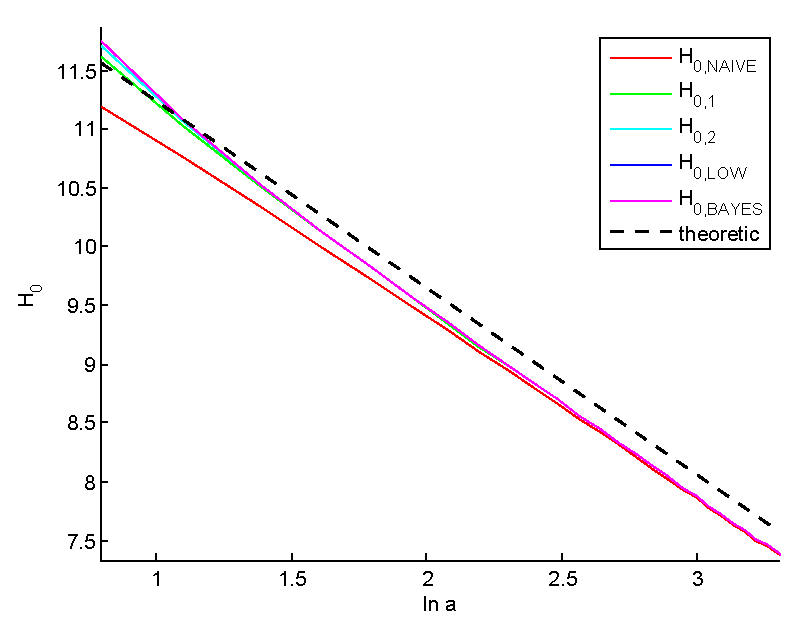
\includegraphics[width=0.4\textwidth]{images5/frac32i.pdf} &
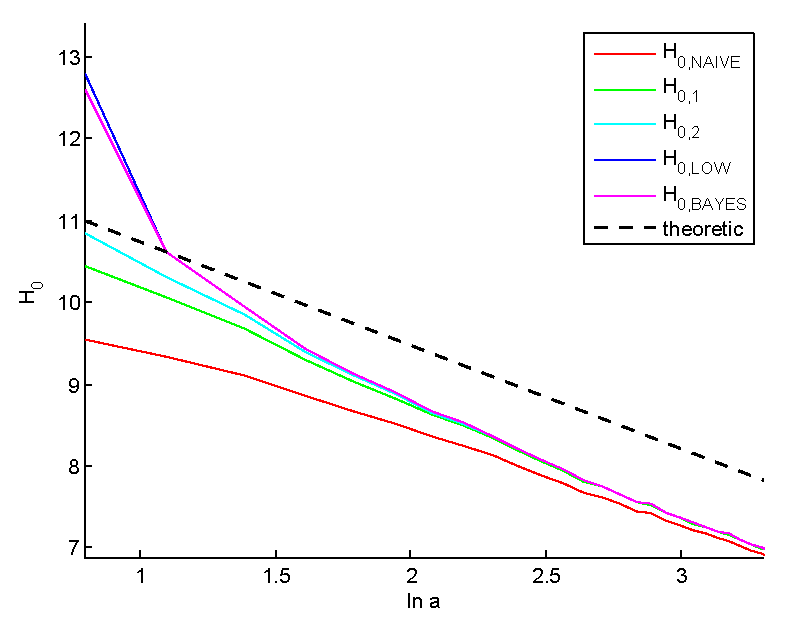
\includegraphics[width=0.4\textwidth]{images5/frac43i.pdf} \\
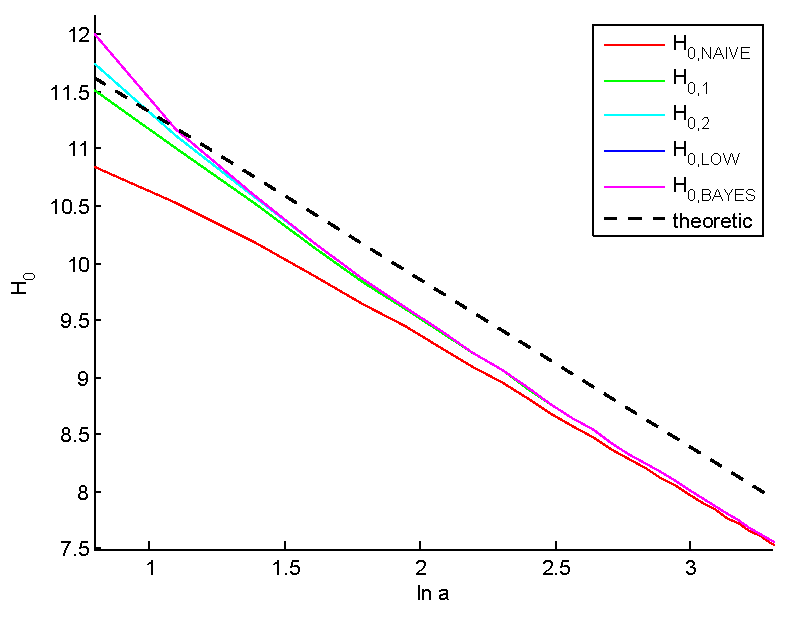
\includegraphics[width=0.4\textwidth]{images5/frac53i.pdf} &
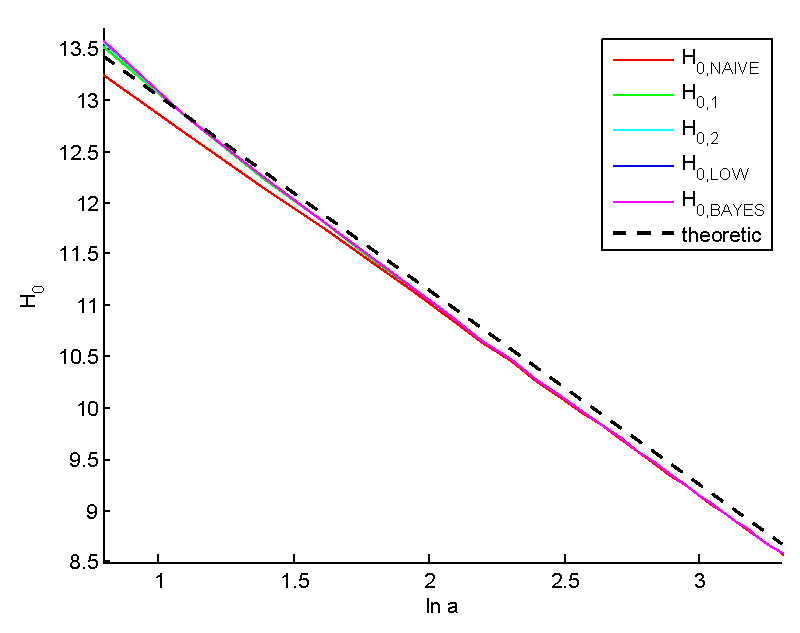
\includegraphics[width=0.4\textwidth]{images5/frac83i.pdf}
\end{tabular}
\caption{Hartley entropy estimates: $F_{32}$ (top left), $F_{43}$ (top right), $F_{53}$ (bottom left), $F_{83}$ (bottom right) }
\label{fig:frac}
\end{figure}


\begin{figure}[H]
\centering
\begin{tabular}{cc}
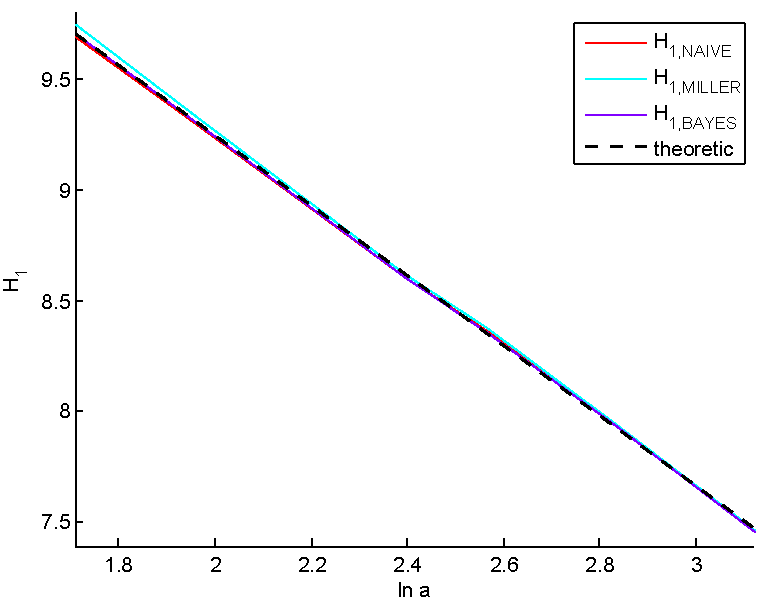
\includegraphics[width=0.4\textwidth]{images4/frac32si.pdf} &
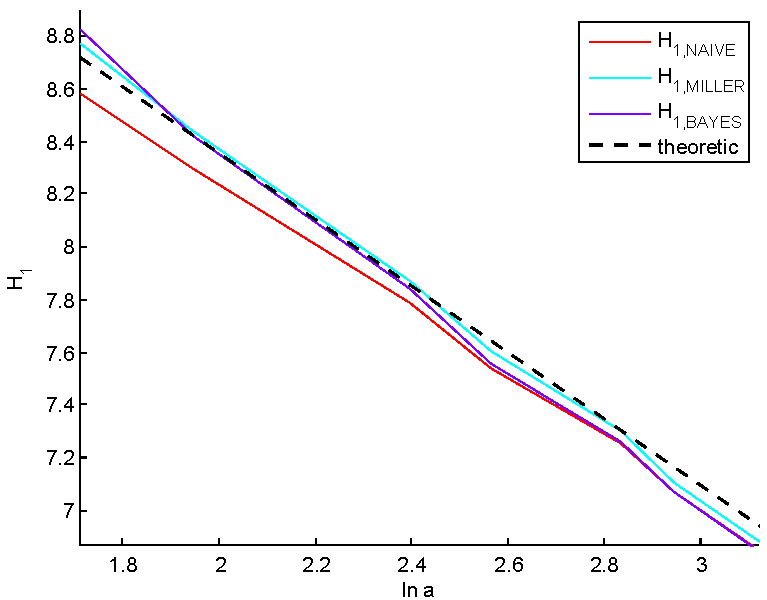
\includegraphics[width=0.4\textwidth]{images4/frac43si.pdf} \\
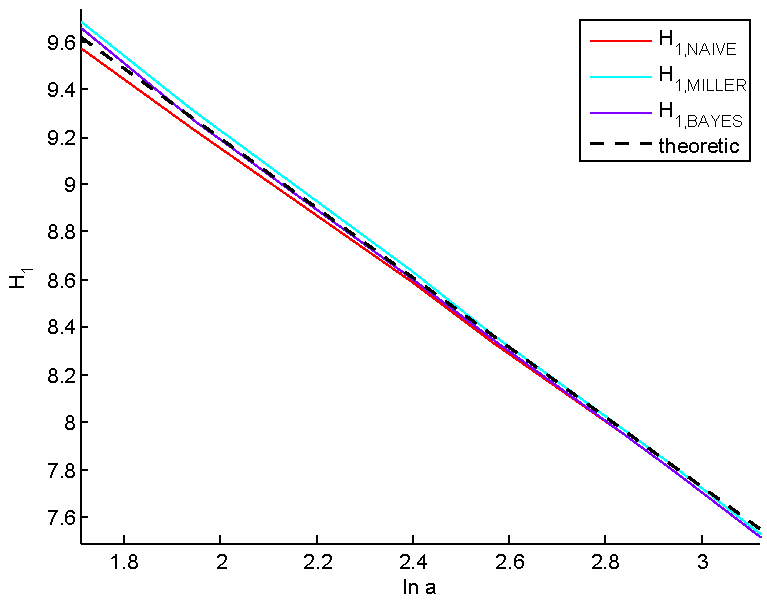
\includegraphics[width=0.4\textwidth]{images4/frac53si.pdf} &
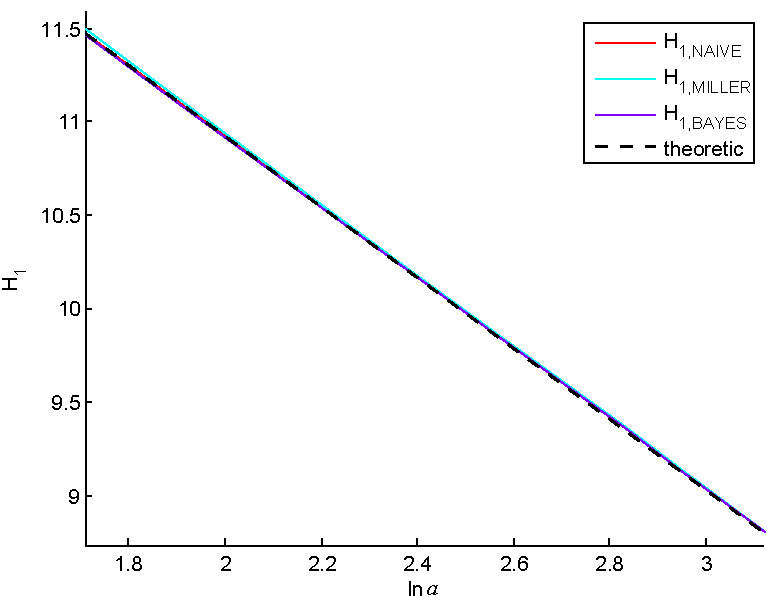
\includegraphics[width=0.4\textwidth]{images4/frac83si.pdf}
\end{tabular}
\caption{Shannon entropy estimates: $F_{32}$ (top left), $F_{43}$ (top right), $F_{53}$ (bottom left), $F_{83}$ (bottom right) }
\label{fig:fracshan}
\end{figure}



\begin{table}[H] 
\begin{center}
\caption{Dimension estimates for $\mathbb{F}_{3,2}$}
\label{tab:est1}
\begin{tabular}{|l|l|l|l|}
\hline
 estimate & \multicolumn{3}{c|}{$\mathbb{F}_{3,2}$} \\
\hline
 & $\hat{D}$ & $s_{D}$ & $z_{\mbox{\scriptsize{score}}}$ \\
\hline 
$ H_{0,\mbox{\scriptsize{NAIVE}}} $ & 1.5714 & 0.0052 & -2.6384 \\ 
\hline 
$ H_{0,1} $ & 1.5765 & 0.0051 & -1.6604 \\ 
\hline 
$ H_{0,2} $ & 1.5765 & 0.0051 & -1.6565 \\ 
\hline 
$ H_{0,\mbox{\scriptsize{LOW}}} $ & 1.5765 & 0.0051 & -1.6565 \\ 
\hline 
$ H_{0,\mbox{\scriptsize{BAYES}}} $ & 1.5765 & 0.0051 & -1.6565 \\ 
\hline 
\end{tabular}
\end{center}
\end{table} 

\begin{table}[H] 
\begin{center}
\caption{Dimension estimates for $\mathbb{F}_{4,3}$}
\label{tab:est2}
\begin{tabular}{|l|l|l|l|}
\hline
 estimate & \multicolumn{3}{c|}{$\mathbb{F}_{4,3}$} \\
\hline
 & $\hat{D}$ & $s_{D}$ & $z_{\mbox{\scriptsize{score}}}$ \\
\hline 
$ H_{0,\mbox{\scriptsize{NAIVE}}} $ & 1.2233 & 0.0136 & -2.8259 \\ 
\hline 
$ H_{0,1} $ & 1.2565 & 0.0135 & -0.3963 \\ 
\hline 
$ H_{0,2} $ & 1.2575 & 0.0135 & -0.3202 \\ 
\hline 
$ H_{0,\mbox{\scriptsize{LOW}}} $ & 1.2576 & 0.0135 & -0.3177 \\ 
\hline 
$ H_{0,\mbox{\scriptsize{BAYES}}} $ & 1.2576 & 0.0135 & -0.3175 \\ 
\hline  
\end{tabular}
\end{center}
\end{table} 

\begin{table}[H] 
\begin{center}
\caption{Dimension estimates for $\mathbb{F}_{5,3}$}
\label{tab:est3}
\begin{tabular}{|l|l|l|l|}
\hline
 estimate & \multicolumn{3}{c|}{$\mathbb{F}_{5,3}$} \\
\hline
 & $\hat{D}$ & $s_{D}$ & $z_{\mbox{\scriptsize{score}}}$ \\
\hline 
$ H_{0,\mbox{\scriptsize{NAIVE}}}  $ & 1.4484 & 0.0082 & -2.0304 \\ 
\hline 
$ H_{0,1} $ & 1.4616 & 0.0081 & -0.4159 \\ 
\hline 
$ H_{0,2} $ & 1.4617 & 0.0081 & -0.3983 \\ 
\hline 
$ H_{0,\mbox{\scriptsize{LOW}}} $ & 1.4617 & 0.0081 & -0.3981 \\ 
\hline 
$ H_{0,\mbox{\scriptsize{BAYES}}} $ & 1.4617 & 0.0081 & -0.3981 \\ 
\hline 
\end{tabular}
\end{center}
\end{table}

\begin{table}[H] 
\begin{center}
\caption{Dimension estimates for $\mathbb{F}_{8,3}$}
\label{tab:est4}
\begin{tabular}{|l|l|l|l|}
\hline
 estimate & \multicolumn{3}{c|}{$\mathbb{F}_{8,3}$} \\
\hline
 & $\hat{D}$ & $s_{D}$ & $z_{\mbox{\scriptsize{score}}}$ \\
\hline
$ H_{0,\mbox{\scriptsize{NAIVE}}} $ & 1.8398 & 0.0040 & -13.0862 \\ 
\hline 
$ H_{0,1} $ & 1.8413 & 0.0042 & -12.4030 \\ 
\hline 
$ H_{0,2} $ & 1.8413 & 0.0042 & -12.4020 \\ 
\hline 
$ H_{0,\mbox{\scriptsize{LOW}}} $ & 1.8413 & 0.0042 & -12.4020 \\ 
\hline 
$ H_{0,\mbox{\scriptsize{BAYES}}} $ & 1.8413 & 0.0042 & -12.4020 \\ 
\hline 
\end{tabular}
\end{center}
\end{table}







\begin{table}[H] 
\begin{center}
\caption{Dimension estimates for $\mathbb{F}_{3,2}$}
\label{tab:est1s}
\begin{tabular}{|l|l|l|l|}
\hline
 estimate & \multicolumn{3}{c|}{$\mathbb{F}_{3,2}$} \\
\hline
 & $\hat{D}$ & $s_{D}$ & $z_{\mbox{\scriptsize{score}}}$ \\
\hline
$ H_{1,\mbox{\scriptsize{NAIVE}}} $ & 1.5797 & 0.0030 & -1.7182 \\ 
\hline 
$ H_{1,\mbox{\scriptsize{MILLER}}} $ & 1.5823 & 0.0031 & -0.8626 \\ 
\hline 
$ H_{1,\mbox{\scriptsize{BAYES}}} $ & 1.5797 & 0.0030 & -1.7155 \\ 
\hline 
\end{tabular}
\end{center}
\end{table}

\begin{table}[H] 
\begin{center}
\caption{Dimension estimates for $\mathbb{F}_{4,3}$}
\label{tab:est2s}
\begin{tabular}{|l|l|l|l|}
\hline
 estimate & \multicolumn{3}{c|}{$\mathbb{F}_{4,3}$} \\
\hline
 & $\hat{D}$ & $s_{D}$ & $z_{\mbox{\scriptsize{score}}}$ \\
\hline 
$ H_{1,\mbox{\scriptsize{NAIVE}}} $ & 1.2698 & 0.0072 & 1.1093 \\ 
\hline 
$ H_{1,\mbox{\scriptsize{MILLER}}} $ & 1.2866 & 0.0069 & 3.5709 \\ 
\hline 
$ H_{1,\mbox{\scriptsize{BAYES}}} $ & 1.2763 & 0.0071 & 2.0192 \\ 
\hline 
\end{tabular}
\end{center}
\end{table}

\begin{table}[H] 
\begin{center}
\caption{Dimension estimates for $\mathbb{F}_{5,3}$}
\label{tab:est3s}
\begin{tabular}{|l|l|l|l|}
\hline
 estimate & \multicolumn{3}{c|}{$\mathbb{F}_{5,3}$} \\
\hline
 & $\hat{D}$ & $s_{D}$ & $z_{\mbox{\scriptsize{score}}}$ \\
\hline 
$ H_{1,\mbox{\scriptsize{NAIVE}}} $ & 1.4691 & 0.0046 & 0.9019 \\ 
\hline 
$ H_{1,\mbox{\scriptsize{MILLER}}} $ & 1.4757 & 0.0048 & 2.2218 \\ 
\hline 
$ H_{1,\mbox{\scriptsize{BAYES}}} $ & 1.4717 & 0.0046 & 1.4442 \\ 
\hline 
\end{tabular}
\end{center}
\end{table}

\begin{table}[H] 
\begin{center}
\caption{Dimension estimates for $\mathbb{F}_{8,3}$}
\label{tab:est4s}
\begin{tabular}{|l|l|l|l|}
\hline
 estimate & \multicolumn{3}{c|}{$\mathbb{F}_{8,3}$} \\
\hline
 & $\hat{D}$ & $s_{D}$ & $z_{\mbox{\scriptsize{score}}}$ \\
\hline
$ H_{1,\mbox{\scriptsize{NAIVE}}}  $ & 1.8641 & 0.0013 & -22.3767 \\ 
\hline 
$ H_{1,\mbox{\scriptsize{MILLER}}} $ & 1.8648 & 0.0013 & -21.1850 \\ 
\hline 
$ H_{1,\mbox{\scriptsize{BAYES}}} $ & 1.8638 & 0.0013 & -22.9511 \\ 
\hline 
\end{tabular}
\end{center}
\end{table}



\newpage



\end{thebibliography}
\begin{appendices}

\section {Appendix}

\subsection {Construction of Bayesian Estimation of Hartley Entropy}

Let $\mathbb{Q}_{n} = \{ \vec{q} \in (\mathbb{R}_{0}^{+})^{n} | \sum_{j=1}^{n}q_{j} = 1 \}$ be support set for uniform random variable $\vec{p} \in \mathbb{Q}_{n}$. Then for integer $K$ satisfying $1 \le K \le \min(n,N)$, the conditional probability is 
\begin{equation} 
\label{eq:probpkn}
\text{p}(K \: | \: n,N) = \text{prob}\left(\sum_{N_{j}>0} 1 = K \: \middle| \: n, \sum_{j=1}^{n}N_{j} = N\right).
\end{equation}
The vector of $N_{j}$ can be reorganized to begin with positive values. Therefore
\begin{equation} 
\label{eq:probbinom}
\text{p}(K \: | \: n,N) = {n \choose K}\text{prob}\left( \forall j=1,...,n : N_{j} > 0 \Leftrightarrow j \le K \: \middle| \: n, \sum_{j=1}^{K}N_{j}=N\right).
\end{equation}
Let $\mathbb{D}_{K,N} = \{ \vec{x} \in \mathbb{N}^K | \sum_{j=1}^{K}x_{j} = N \}$ be domain of $\vec{N} = (N_{1},...,N_{K}) \in \mathbb{D}_{K,N}$. Using mean value of multinomial distribution over $\mathbb{Q}_{n}$, we obtain
\begin{equation} 
\label{eq:probbinomexp}
\text{p}(K \: | \: n,N) = {n \choose K} \text{E}\left(\sum_{\vec{N} \in \mathbb{D}_{K,N}} {N \choose N_{1},...,N_{K}} \prod_{j=1}^{K}p_{j}^{N_{j}} \prod_{j=k+1}^{n}p_{j}^{0} \right) = {n \choose K} \text{E}\left(\sum_{\vec{N} \in \mathbb{D}_{K,N}} {N \choose N_{1},...,N_{K}} \text{E}\prod_{j=1}^{K}p_{j}^{N_{j}}\right).
\end{equation}
Using generalized Beta function
\begin{equation} 
\label{eq:betafce}
B(\vec{x}) = \int_{\vec{p} \in \mathbb{Q}_{m}} \prod_{j=1}^{m} p_{j}^{x_{j}-1} \text{d}\vec{p} = \frac{\prod_{j=1}^{m} \Gamma(x_{j})}{\Gamma(\sum_{j=1}^{m}x_{j})},
\end{equation}
we can calculate
\begin{equation} 
\label{eq:expprod}
\text{E}(\prod_{j=1}^{K}p_{j}^{N_{j}}) = \frac{\int_{\vec{p} \in \mathbb{Q}_{n}} \prod_{j=1}^{K} p_{j}^{N_{j}} \text{d}\vec{p}}{\int_{\vec{p} \in \mathbb{Q}_{n}} \text{d}\vec{p}} = \frac{\prod_{j=1}^{K}\Gamma(N_{j}+1)}{\Gamma(N+n)}
\end{equation}
Therefore
\begin{equation} 
\label{eq:prob}
\text{prob}(K \: | \: n,N) = {n \choose K}\sum_{\vec{N} \in \mathbb{D}_{K,N}} \frac{N!(n-1)!}{\prod_{j=1}^{K}N_{j}!}\frac{\prod_{j=1}^{K}N_{j}!}{(N+n-1)!} = {n \choose K}\sum_{\vec{N} \in \mathbb{D}_{K,N}} \frac{N!(n-1)!}{(N+n-1)!} = \frac{{n \choose K}\text{card}(\mathbb{D}_{K,N})}{{N+n-1 \choose n-1}}.
\end{equation}
The last question is about the cardinality of $\mathbb{D}_{K,N}$, which corresponds with number of possibilities, how to place $N$ balls into $K$ boxes under assumptions that no box is empty and the balls are identic. We place $K$ balls into $K$ different boxes in the first phase. The rest of $N-K$ balls can be distributed without any constrains. Therefore
\begin{equation} 
\label{eq:card}
\text{card}(\mathbb{D}_{K,n}) = {(N-K)+K-1 \choose K-1} = {N-1 \choose K-1}. 
\end{equation}
Resulting formula is (\ref{eq:pknn}).



\subsection{Matlab library}

\subsubsection{Bayesian estimate $ H_{0,\mbox{\scriptsize{BAYES}}}$ }
\ttfamily
\begin{lstlisting}
function H0=HARTLEYBAYES(N,k,nmax)
    nstar=1e7;
    tol=1e200; 
    if nargin == 1
        nmax=length(N);
        k=sum(N>0);
        Ntotal=sum(N);
    else
        Ntotal=N;
    end
    if nargin==2
        nmax=nstar;
    end
    if k>Ntotal-2 && nmax==nstar
        H0=NaN;
        return
    end
    bay=1;
    bay0=log(k);
    b=1;
    H0=bay0/bay;
    for j=1:nmax-k
        H0old=H0;
        b=b/j*(k+j)*(k+j-1)/(k+Ntotal+j-1);
        bay=bay+b;
        bay0=bay0+b*log(k+j);
        H0=bay0/bay;
        if bay>tol
            bay0=bay0/bay;
            b=b/bay;
            bay=1;
        end
        if abs(H0-H0old)< 1e-8
            break
        end
    end
end
\end{lstlisting}

\normalfont
\subsubsection{Bayesian estimate $ H_{1,\mbox{\scriptsize{BAYES}}}$ }
\ttfamily
\begin{lstlisting}
function H1=SHANNONBAYES(N)
    nstar=1e7;
    tol=1e200; 
    Ntotal=sum(N);
    nmax=length(N);
    k=sum(N>0);
    N=N(N>0);
    if k>Ntotal-2 && nmax==nstar
        H1=NaN;
        return
    end
    bay=1;
    bay1=SHANNONFIXED(N);
    b=1;
    H1=bay1/bay;
    for j=1:nmax-k
        H1old=H1;
        b=b/j*(k+j)*(k+j-1)/(k+Ntotal+j-1);
        bay=bay+b;
        N=[N,0];
        bay1=bay1+b*SHANNONFIXED(N);
        H1=bay1/bay;
        if bay>tol
            bay1=bay1/bay;
            b=b/bay;
            bay=1;
        end
        if abs(H1-H1old)< 1e-8
            break
        end
    end
end
\end{lstlisting}

\normalfont
\subsubsection{Bayesian estimate $ H_{1,\text{n}}$ }
\ttfamily
\begin{lstlisting}
function H1=SHANNONFIXED(N)
	Ntotal=sum(N);
	n=length(N);
	H1=(N+1)/(Ntotal+n)*(psi(Ntotal+n+1)-psi(N+2))';
end
\end{lstlisting}

\normalfont
\ttfamily
\begin{lstlisting}

\end{lstlisting}


\end{appendices}

\end{document}
